\section{Triangulation}
\label{section:triangulation}
We start with leaving the time-derivative untouched, and focus on the discretization in space for now - we are performing a \textit{space semidiscretization}.
\paragraph{}
First step in the process of the discretization is to divide the computational domain $\overline{\Omega}$ into a finite number of subsets with properties described below. These subsets form the set, further denoted by $ T_h$, called the \textit{triangulation or mesh of the domain $\Omega$}. Please note that the terms \textit{triangulation} and \textit{mesh} shall be used in the text interchangeably. The parameter $h>0$ of the triangulation usually represents maximum of diameters of all elements $K\in T_h$. The elements $K\in T_h$ are in the context of the finite volume method called $finite\ volumes$.
\\\ \\Properties of $T_h$:
\begin{enumerate}
    \item Each $K\in T_h$ is closed and connected with its interior $K^{\circ}\neq\emptyset$.
    \item Each $K\in T_h$ has a Lipschitz boundary.
    \item$\cup_{K\in T_h}K\,=\,\overline{\Omega}$
    \item If $K_1,K_2\in T_h$, $K_1\neq{K_2}$, then $K_1^{\circ}\cap{T}_2^{\circ} = \emptyset$.
\end{enumerate}
\paragraph{}
In our case of the three-dimensional problem, we assume that the domain $\Omega$ is obtained as an approximation of the original computational domain (also denoted by $\Omega$), and the triangulation is chosen accordingly to the following attributes:
\renewcommand{\labelenumi}{\Alph{enumi})}
\begin{enumerate}
    \item Each $K\in T_h$ is a closed rectangular hexahedron, possibly with curved faces.
    \item For $K_1,K_2\in T_h,\,K_1\neq{K}_2$ we have either $K_1\cap{K}_2 = \emptyset$ or $K_1,K_2$ share one face (if the shared face is a whole common face, we call the triangulation \emph{regular}), or $K_1,K_2$ share one vertex, or $K_1,K_2$ share one face.
    \item$\cup_{K\in T_h}K\,=\,\overline{\Omega}.$
\end{enumerate}
Furthermore
\be
\label{Idef}  T_h = \left\{K^i, i\in I\right\},
\ee
where $I\subset Z^+ = \left\{0, 1, 2, ...\right\}$ is a suitable index set.\\
By $\Gamma_{ij}$ we denote a common face between two
neighboring elements $K^i$ and $K^j$. We set 
$$s
\lo i\ro = \left\{j\in I; K^j \text{ is adjacent to } K^i\right\}.
$$
The boundary $\partial\Omega$ is formed by a finite number of faces of elements $K^i$ adjecent to
$\partial\Omega$. We denote all these boundary faces by $S_j$, where $j\in I_b\subset Z^{-} = \left\{-1, -2, ...\right\}$.
Now we set 
$$
\gamma\lo i \ro = \left\{j\in I_b; S_j \text{ is a face of } K^i\in T_h\right\}
$$ 
and 
$$
\Gamma_{ij} = S_j\text{ for } K^i\in  T_h\text{ such that }S_j\subset\partial K^i, j\in I_b.
$$
For $K^i$ not containing any boundary face $S_j$ we set $\gamma\lo i \ro = \emptyset$.\\
Obviously, $s\lo i \ro \cap\gamma\lo i\ro = \emptyset$ for all $i\in I$. If we write $S\lo i \ro = s \lo i\ro \cup \gamma\lo i \ro$, we have
$$
\partial K^i = \cup_{j\in S\lo i \ro}\Gamma_{ij},\ \ \ \partial K^i\cap\partial{\Omega} = \cup_{j\in\gamma\lo i \ro}\Gamma_{ij}.
$$
Furthermore we define the set of internal (i.e. not lying on the boundary $\partial\Omega$) faces as
\be
\label{InternalEdges} \Gamma_I = \cup_{i\in I} \cup_{j \notin \gamma\lo i \ro} \Gamma_{ij},
\ee
and the set of boundary (i.e. lying on the boundary $\partial\Omega$) faces as
\be
\label{BndEdges} \Gamma_B = \cup_{i\in I} \cup_{j \in \gamma\lo i \ro} \Gamma_{ij}.
\ee
\paragraph{Note}
If we were to use not $\Omega\subset\mathbb{R}^3$, but rather $\Omega\subset\mathbb{R}^4$, we may just employ the following machinery also to the time-derivative - this is not an uncommon approach. Why the approach described in this work is favored by the author is twofold:
\begin{itemize}
    \item Data (in a general sense - e.g. algebraic systems, function bases, etc.) are smaller when using a separate handling for time-derivative
    \item The dependency on time and space may (and usually does) vary a lot for physical phenomena - to have a separate approach is therefore beneficial
\end{itemize}
\subsection{Distributed triangulation}
\label{section:ditributedTria}
The standard approach to handle large problems that are impossible to be calculated on a single processor in mesh-based numerical simulations (such as Discontinuous Galerkin method) is to employ a \textit{domain decomposition} method, where each of the processors on which the simulation runs holds data about a subset of elements of the mesh $T$.
Consequently, also the matrix and vector assembly (described in ~\Cref{algorithm:singleTimeStep}), the linear problem solution, slope limiting, and AMR procedures are performed by all processors using data they have available. The aim here is not to go into deep technical details of distributing data, etc.
\paragraph{}
In \Crefrange{figure:domainDecomposition}{figure:domainDecomposition2}, domain $\Omega = \left[0, 1\right] \times \left[0, 1\right] \times \left[0, 1\right]$ was used, it was triangulated by $10 \times 10 \times 10$ mesh elements and the domain was distributed among 5 processors labelled $0..4$.

\begin{figure}[H]
		\begin{center}
			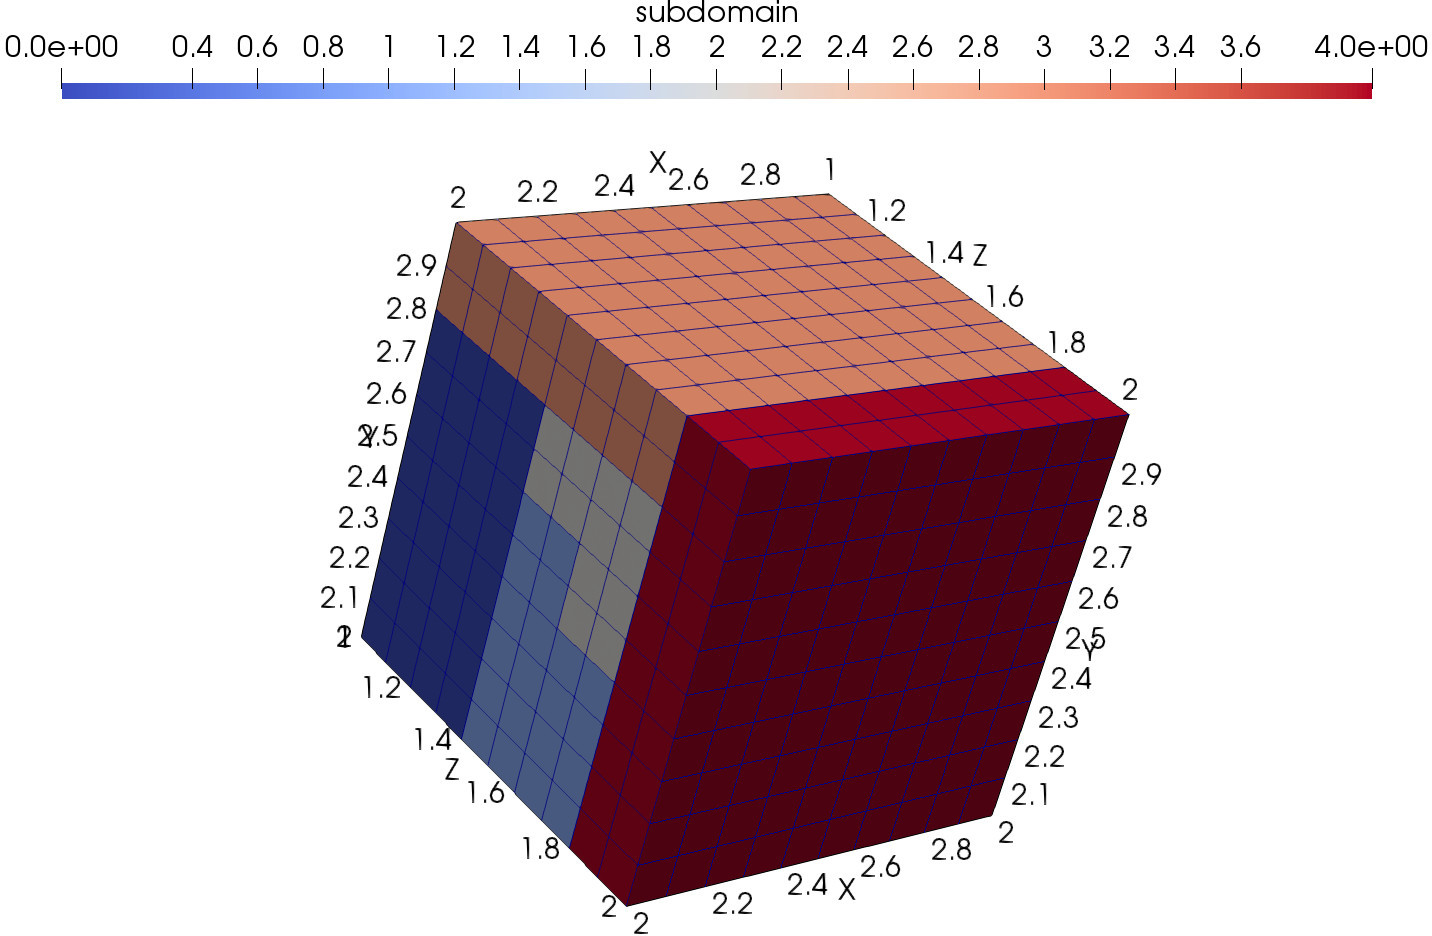
\includegraphics[width=0.78\textwidth]{img/mesh/cube.jpg}
			\vspace{-2mm}
		\caption{Cubical domain $\Omega$ with color-coded processor-owned elements.}
		\label{figure:domainDecomposition}
		\end{center}
	\end{figure}\vspace{-5mm}
	
\begin{figure}[H]
		\begin{center}
			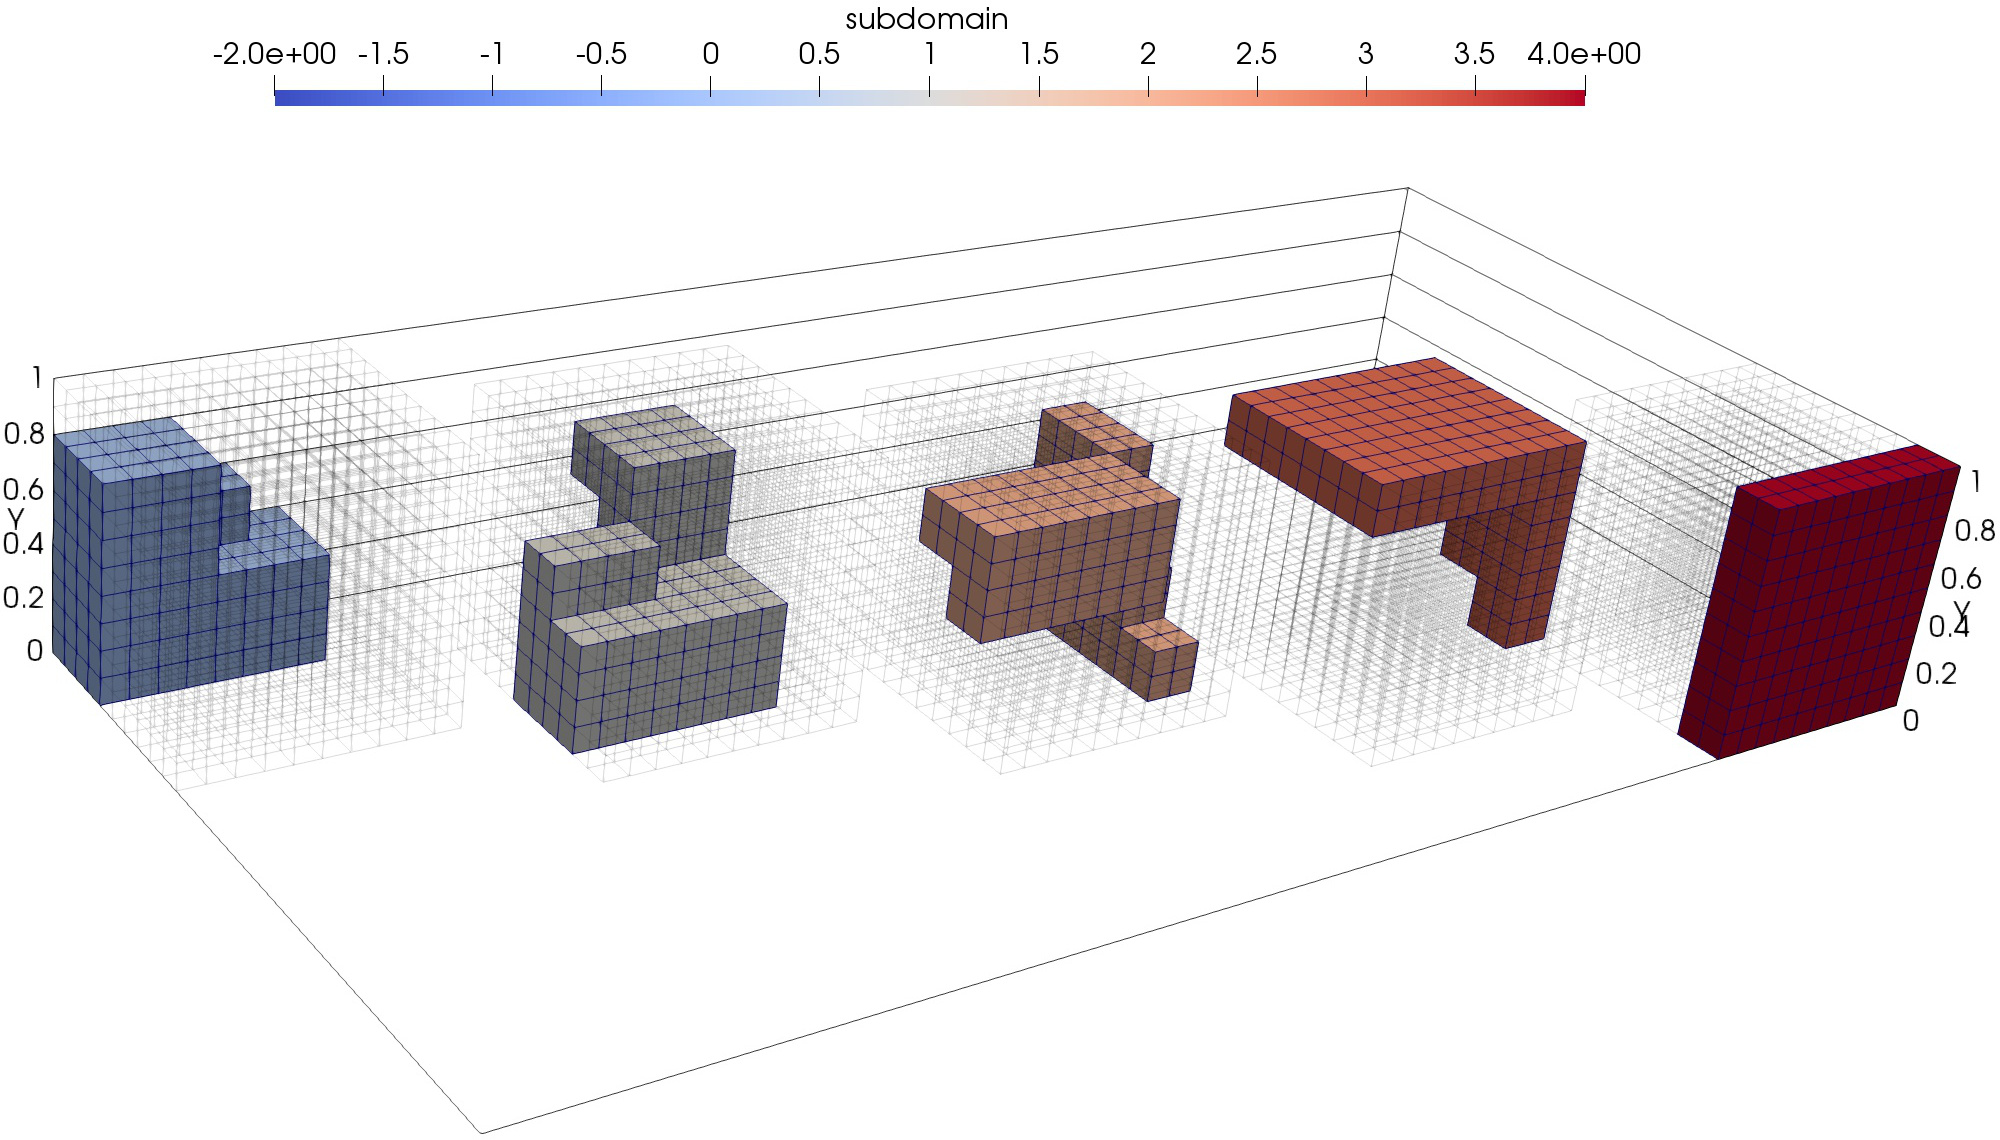
\includegraphics[width=0.78\textwidth]{img/mesh/cubeSub.jpg}
			\vspace{-2mm}
		\caption{The same domain as in \Cref{figure:domainDecomposition}, with clearer indication of elements that belong to individual processors (0..4 left to right).}
		\label{figure:domainDecomposition2}
		\end{center}
	\end{figure}\vspace{-5mm}
	